% DIAGNOSIS
%
% !TEX root = ../thesis-main.tex
%
\chapter{Diagnosis of lexical stress errors}
\label{chap:diagnosis}

%\cleanchapterquote{You can’t do better design with a computer, but you can speed up your work enormously.}{Wim Crouwel}{(Graphic designer and typographer)}

In order to provide learners with useful feedback on their lexical stress errors in the L2, 
the prototype CAPT tool developed in this thesis project 
must first be able to automatically detect and diagnose such errors in a learner's utterance. This requires at least:
\begin{enumerate}[label=(\alph*)]
\item Reasonably accurate word-, syllable- and phone-level segmentation of the learner's L2 utterance; 
\item %A means of analyzing
An analysis of how lexical stress is realized in the
% prosody of the segmented 
given
utterance;
\item A representation of how native speakers of the target language (would) realize lexical stress in the given sentence; and
\item %A way of comparing
A comparison of the learner's prosody to this representation. 
\end{enumerate}

This chapter describes 
%
how (a) is achieved using
 forced-alignment segmentation of a learner's read-speech utterance with the corresponding text, 
 %and how problems in accuracy of the resulting segmentation can be overcome 
 (\cref{sec:diag:segmentation}); 
 %
 how the lexical stress analysis of (b), which is also crucial to (c), is produced by measuring the fundamental frequency, duration, and energy of relevant sections of the speech signal (\cref{sec:diag:prosody}); 
 %
 and finally, the various approaches to (c) and (d) that are implemented in the prototype tool, and how the system's modular architecture allows researchers and teachers control over which of these approaches are used \TODO{\textit{update section organization?} (\cref{sec:diag:compare})}.



\section{Automatic segmentation of nonnative speech}
\label{sec:diag:segmentation}

%Automatic 
Segmentation, or labeling, of a recorded utterance is the task of annotating the speech signal with boundaries that demarcate individual phones, syllables, words, sentences, and/or other units of speech; see \cref{fig:GGsegmentation} for an example of a multi-level segmentation of a German utterance. 
	
	\begin{figure}
		\centering
		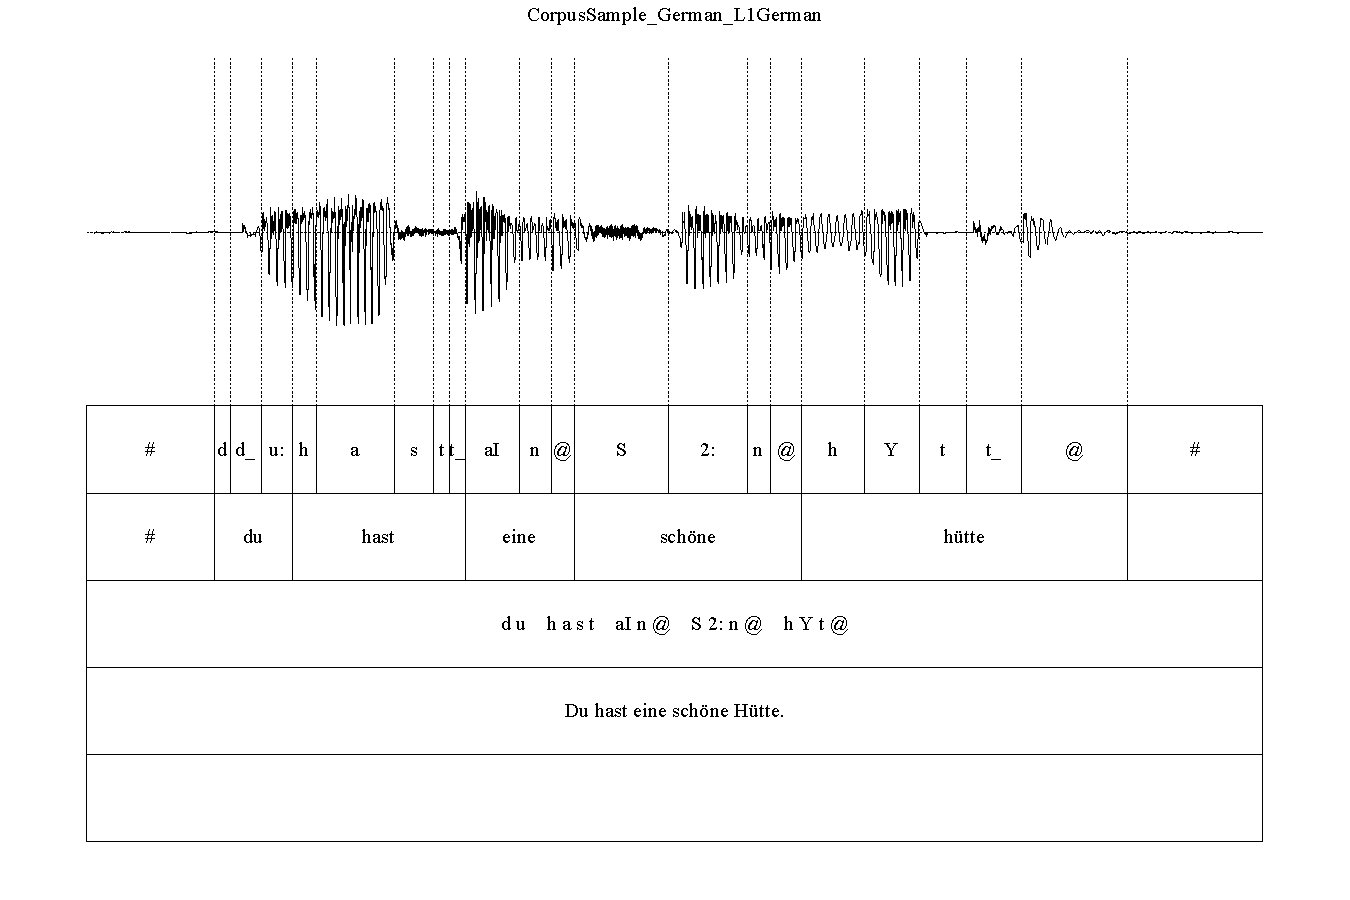
\includegraphics[width=\textwidth]{img/screenshots/SampleGG-basic}
		\caption[An example German utterance and its segmentation]{\TODO{update with new example w/ SyllableTier} An example of a German utterance that has been segmented at the phone level (first row) and word level (second row). The third row contains the canonical (expected) native pronunciation of each word in the sentence, while the fourth row contains the written sentence of which the utterance is a reading.}
		\label{fig:GGsegmentation}
	\end{figure}


A reasonably accurate segmentation of an L2 learner's utterance is indispensable for an analysis of the accuracy of their pronunciation; 
\TODO{mention that there are methods which don't need segmentation, but they're more limited?}
as it allows comparison between relevant units of the learner's utterance -- e.g. words, syllables, and phones -- and corresponding units in native speech. 
The most accurate segmentation would of course be one produced by hand by a trained phonetician. However, hand-labeling is not feasible in most scenarios because of its high cost in terms of time and wages; moreover, because the ultimate goal of this work is the development of a CAPT tool which can give L2 learners helpful automatic feedback on their pronunciation, 
%even when they do not have access to a language teacher, 
any analysis of the learner's speech signal, including the preliminary step of segmentation, must proceed fully automatically. Therefore, a means of automatically segmenting a given utterance is required.



	%\subsection{Segmentation via forced alignment}
	%\label{sec:segmentation:alignment}
	
	When the content (text) of a given utterance is already known, the goal of automatic segmentation becomes aligning the  boundaries of each phone in the expected sentence with the appropriate points in the recorded signal. Boundaries for larger units such as syllables and words can be inferred from the phone boundaries. 
	An effective and widely-used technique for this is forced alignment \citep{Fohr1996,Mesbahi2011}, 
	which \TODO{...}
	%
	This technique 
	requires 
%knowledge of the text of the given utterance (known beforehand in the IFCASL case), 
	the expected text of the given utterance, 
	acoustic models of the target language, and a pronunciation lexicon that describes the sequence of phones expected for each word. To account for differences in how different speakers (especially non-native speakers) may pronounce the given sentence, 
	%the lexicon is supplemented with a lexicon of non-native pronunciation variants 
	the lexicon should contain not only the canonical pronunciation for each word, i.e. the pronunciation that might be given in a standard dictionary, but also any alternate or non-standard pronunciation variants (native or non-native) that might be encountered. 	
	
	
	\TODO{mention how a real CAPT system would have to do this on the fly, and that can be done in Jsnoori, but the prototype assumes segmentation has been done and mocks that up by only using auto segmentations of IFCASL data}
	
	The native and non-native read speech recordings comprising the IFCASL corpus \citep{Fauth2014,Trouvain2013} have been automatically segmented via forced alignment 
	\citep{Fohr1996,Mesbahi2011}.
%(see e.g. \cite{Fohr1996,Mesbahi2011}). 
	
	
%TODO is it worth mentioning retraining the AMs? will I actually try that?
%	In the segmentation of the German IFCASL subcorpus, the acoustic models used have been trained on native German speech data. 
	
	The IFCASL corpus uses segmentations at the phone and word levels, 
	but not at the syllable level.
	%and a subset of these automatic segmentations has been manually verified.
	As the syllable is arguably the most important unit for analysis of lexical stress realization \TODO{reference/justification}, syllable-level segmentations for each utterance had to be added. This was accomplished by 
	 %However, segmentation at the syllable level still needs to be performed. This may be accomplished based on the word- and phone-level annotations by automatically or 
	 manually determining the phones between which syllable boundaries are expected in each sentence from the text and phonetic lexicon, 
	\TODO{using the syllabification program [...] and a pronunciation dictionary?}.
	 Given the sequence of phones expected for each syllable, the locations of syllable boundaries were automatically extracted from the phone-level segmentation, and automatically combined with the word-level boundaries to create the syllable-level segmentation. 
	

	
	%\subsection{Evaluation of segmentation accuracy}
	%\label{sec:segmentation:eval}
	\TODO{xxxxxxxxxxxxxxxxxxxx}
	
	The accuracy of the forced-alignment segmentation can be assessed by computing inter-annotator agreement between the automatically produced segmentation and one or more manually-verified segmentations. The team at LORIA in Nancy has already completed this evaluation for the French IFCASL sub-corpus using the CoALT tool \citep{Fohr2012}. In cooperation with that team, the German sub-corpus (or a subset thereof) will be evaluated in the same way.
	A similar evaluation will be carried out for the syllable-level segmentations, a subset of which will be manually verified.

%	Error analysis will be performed for each boundary type, to enable identification of the types of boundaries at which the system tends (not) to make many errors. This detailed analysis will contribute to error management in the system, as described 
%in \cref{sec:segmentation:errors}.
%below.


%%%%%%%%%%%%%%%%%%%%%%%
%%% Moved to Future Work
%%%%%%%%%%%%%%%%%%%%%%%
%	\subsection{Coping with segmentation errors}
%	\label{sec:segmentation:errors}
%	
%	Forced alignment is not a perfect method; because of the constraints put on the recognition system, the aligner will always find a match between the given text and audio, even if they do not correspond. Incorrect segmentation can lead to mistakes in diagnosis, so CAPT systems must have a means of reducing, or at least monitoring, the amount of error introduced by inaccurate segmentation \citep{Eskenazi2009}. 	
%	In the proposed CAPT tool, this function may be served by the development of a simple sentence- and/or word-level confidence measure. 
%	While it is very difficult to compute such a measure directly from the decoding scores of the forced aligner, it may be possible to determine from the aforementioned accuracy evaluation which types of boundaries (e.g. between a sonorant and a vowel) the aligner typically has trouble detecting accurately, and then to calculate, for a given utterance, the proportion of error-prone boundaries. While a very simplistic measure, this could nevertheless provide some indication of when (not) to trust the automatic alignment, thus impacting decisions on how and whether to attempt error diagnosis (or feedback).
%	% based on the boundary error rates found in \cref{sec:segmentation:eval}. 
%	Other error-management strategies may also be explored, such as the type of error-filtering methods described by \textcite{Mesbahi2011,Bonneau2012,Orosanu2012}, in which utterances which do not correspond to the expected text are detected and rejected before alignment is attempted.
%%%%%%%%%%%%%%%%%%%%%%%
	
\section{Analysis of word prosody}
\label{sec:diag:prosody}
	
	\TODO{transition}

	This section describes the features by which the system analyzes the lexical stress prosody of an utterance, be it the utterance of a learner or of a native speaker. These features relate to the three \TODO{acoustic properties (and by extension their perceptual correlates)} described in \cref{sec:bkgd:stress}, namely duration (timing), fundamental frequency or F0 (pitch), and intensity (loudness). 
		%The features computed for each property are described in the corresponding sections below.
%
	\TODO{Where possible, the diagnosis module of the CAPT tool will provide researchers control over the features used; for example, there may be an option to include all F0 and duration features but ignore intensity features.}
%	


	Throughout this section, the features discussed are illustrated with their values for a word from \TODO{\textit{three?} two sample utterances} of a German word selected from the IFCASL corpus; one by a L1 French speaker and the other by a L1 German speaker. The oscillogram, waveform, and annotation for these samples are shown in \cref{fig:featuresexample}.
	
	\begin{figure}
		\centering
		\begin{subfigure}[t]{\textwidth}
                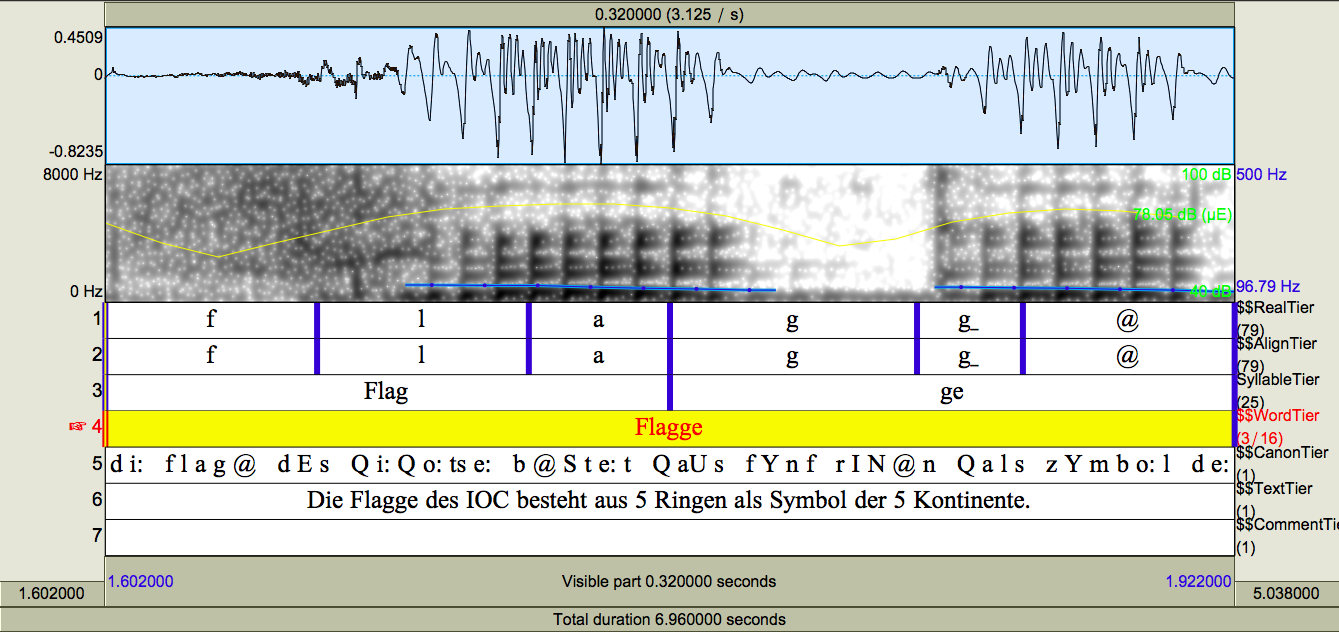
\includegraphics[width=\textwidth]{img/screenshots/2SH05_FGMB1_527-flagge}
                \caption{L1 French speaker (F)}
                \label{fig:featuresexample:fg}
        \end{subfigure}%
        \vspace{1.5em}
        \TODO{Add incorrect FG example?}        \vspace{1.5em}

        \begin{subfigure}[b]{\textwidth}
                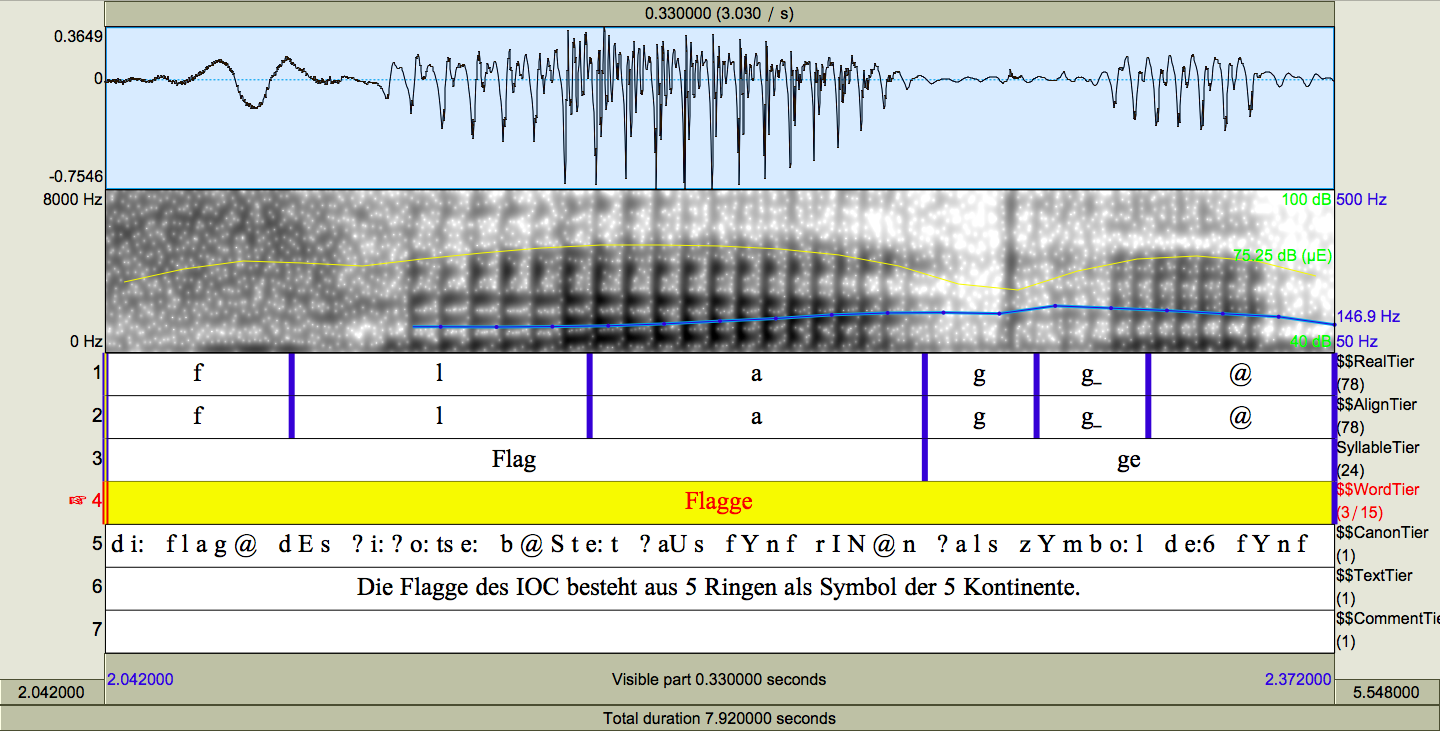
\includegraphics[width=\textwidth]{img/screenshots/2SH05_GGMB2_035-flagge}
                \caption{L1 German speaker (G)}
                \label{fig:featuresexample:gg}
        \end{subfigure}%
		\caption{Two sample utterances of the word "Flagge" from the IFCASL corpus, used to illustrate the features discussed in this section. \TODO{description}}
		\label{fig:featuresexample}
	\end{figure}
	
In this work, the features described below have been computed from the automatically generated segmentation of an utterance \TODO{(see section X)}, and not from a hand-corrected segmentation; as a result, the computed values may be slightly (or in some cases, significantly) inaccurate due to errors in the forced-alignment segmentation process. This reliance only on automatically-detected segment boundaries is intentional, as it simulates the conditions of an automatic, real-time tutoring system, which would need to perform segmentation on the fly and would not have recourse to human verification of segment boundary locations.

	A potential complication of this analysis that should be pointed out relates to the fact that we are here dealing exclusively with read, and not sponaneous, speech. As \textcite[p.~275]{Cutler2005} remarks, ``acoustic differences between stressed and unstressed syllables are relatively large in spontaneous speech. With laboratory-read materials, however, such differences do not always arise''. Therefore, the task of recognizing prosodic deviations in learners' read speech may be somewhat different than the corresponding task for spontaneous speech, and this difference should be kept in mind in the discussion that follows.

	\subsection{Duration}
	\label{sec:prosody:duration}
	%TODO more text
	Analysis of duration (timing) is extremely important for detecting stress patterns;
indeed, syllable duration may be the most important acoustic correlate of lexical stress in German \citep{Dogil1999}.
%as discussed in section %TODO above.
%In this work, duration analysis will figure prominently, and following \textcite{Bonneau2011} will most likely take into account the relative duration of each syllable of the word in question, and/or of the vowel at the nucleus of each syllable. %Other features may also be explored.
Duration analysis therefore figures prominently in the analysis and assessment of learners' lexical stress in this work. Following \textcite{Bonneau2011}, we take into account the relative duration of each syllable of the word to be analyzed, as well as the relative duration of the vowels at the nucleus of each syllable. 
The complete list of features computed for each utterance is given in \cref{tab:durationfeatures}, 
%TODO 
along with the values computed for a sample utterance from the IFCASL corpus \TODO{reference?}. 



\begin{table}[htb]
		\centering
		\caption[Features computed for duration analysis]{Features computed for duration analysis, and their values for the sample utterances of ``Flagge'' in \cref{fig:featuresexample}. Values are given in seconds.}
		\begin{tabularx}{\textwidth}{lXcc}
		\toprule
		\multirow{2}{*}{Feature name} 
									& \multirow{2}{*}{Description}
																	& \multicolumn{2}{c}{Value (seconds)} \\
					  				&												&  (a) F		& (b) G \\
		\midrule
		WORD-DUR 		&	Duration of entire word				& 0.32			& 0.33			\\
		SYLL0-DUR 		&	Dur. of 1st syllable						& 0.16			& 0.22			\\
		SYLL1-DUR 		&	Dur. of 2nd syllable				& 0.16			& 0.11			\\
		V0-DUR 				&	Dur. of vowel in 1st syllable		& 0.04			& 0.09			\\
		V1-DUR 				&	Dur. of vowel in 2nd syllable	& 0.06			& 0.05			\\
		SYLL-REL-DUR 	&	SYLL0-DUR$/$SYLL1-DUR 		& 1.00			& 2.00			\\
		V-REL-DUR 		&	V0-DUR$/$V1-DUR					& 0.67			& 1.80 			\\
		\bottomrule	
		\end{tabularx}
		\label{tab:durationfeatures}
\end{table}

The relative utility of these features in automatically diagnosing lexical stress errors is discussed further in \cref{sec:diag:eval}.


	\subsection{Fundamental frequency}
	\label{sec:prosody:f0}
	
	As described in \cref{sec:bkgd:stress}, the fundamental frequency (F0) of an utterance, which corresponds at the perceptual level to its pitch, also provides a strong indication of how lexical stress is realized in that utterance, and F0 features 
	%should therefore also contribute to 
	are another crucial component of
	the system's prosodic analysis. 
	%
	
		\TODO{Pitch in Jsnoori:
	\begin{itemize}
		\item Martin's basic spectral comb algo
		\item with Yves' improvement using parabolic interpolation
		\item with Secrest \& Doddington's improvement for voicing decision 
		\item With dynamic programming (Ney?) to select which F0 values to accept
		\item Soon to implement Yin's temporal method, and then combine results with those of Martin's or another spectral method such as SWIPE (SWYPE?) (combining with NNs or something else)
	\end{itemize}	
	}	
	
	The F0 contour of a given utterance is determined using the pitch detection algorithm(s) implemented in Jsnoori \TODO{ref}. At the heart of Jsnoori's approach to pitch detection lies the algorithm developed by Martin \cref{Martin1982}, which 
	
	\TODO{de-proposal-ize this paragraph}
	Much of the work on assessing non-native lexical stress has been conducted with English as the L2, and thus often makes the assumption that a stressed syllable should have a higher F0 than unstressed syllables \citep{Bonneau2011}. In German, the F0 of a stressed syllable also tends to differ from the surrounding contour, but the difference may be positive (the stressed syllable has a higher pitch) or negative (lower pitch) \citep[p.~267]{Cutler2005}. Therefore, features used to represent F0 may include the absolute value of the difference in average F0 between each pair of adjacent syllables in the word, or perhaps between the syllable which should carry (primary) stress and the rest of the word. To guard against unvoiced segments interfering with the F0 analysis, syllables may be represented by the vowels that form their nuclei. Relative differences between syllables may be more helpful than absolute differences. The F0 variation (range) over the entire word might also be informative of whether or not the speaker failed to stress any syllable.%, although it would not tell us which syllable were stressed. 
	%Other features may be drawn from related work on lexical stress in learner speech, such as \textcite{Bonneau2011}.
	
		%``...in German utterances, stressed syllables could be signaled by any F0 obtrusion from the overall contour, so that a stressed syllable could be either higher or lower in pitch than its neighbors'' \citep[p.~267]{Cutler2005}

		%\setlength\extrarowheight{5pt}
\begin{table}[htb]
		\centering
		\caption[Features computed for fundamental frequency (F0) analysis]{Features computed for fundamental frequency (F0) analysis, and their values for the sample utterances of ``Flagge'' in \cref{fig:featuresexample}. Values are given in semitones.}
		{\renewcommand{\arraystretch}{1.4}%
		\begin{tabularx}{\textwidth}{p{.225\textwidth}Xrr}
		\toprule
		\multirow{3}{*}{Feature name} 
									& \multirow{3}{*}{Description}
																	& \multicolumn{2}{c}{Value} \\
									&								& \multicolumn{2}{c}{(semitones)} \\							
					  				&																	&  (a) F		
					  																											& (b) G
					  																																\\
		\midrule
		%%%% WORD FEATURES 
		WORD-F0-MEAN	& Average (Avg.) F0, entire word	 				& 8.78		& 16.36\\
		WORD-F0-MAX	& Maximum (Max.) F0, entire word				& 10.73	& 20.08\\
		WORD-F0-MIN		& Minimum (Min.) F0, entire word				& 6.27		& 13.65\\
		WORD-F0-RANGE & WORD-F0-MAX$-$WORD-F0-MIN			& 4.46		& 6.43\\
%		WORD-F0-RANGE & {\renewcommand{\arraystretch}{.9}%
%										$\displaystyle\begin{array}{l}%
%										\phantom{-}\mbox{WORD-F0-MAX}\\%
%										-\mbox{WORD-F0-MIN}\\\end{array}$}	& 4.46	& 6.43\\
%		\multirow{2}{*}{WORD-F0-RANGE}	
%									& $\phantom{- }\text{WORD-F0-MAX}$
%																			& \multirow{2}{*}{4.459217}		
%																									& \multirow{2}{*}{6.425775}\\
%									& $- \text{WORD-F0-MIN}$						& 						& 					\\		

		%\addlinespace
		%%%% SYLL* FEATURES 
		SYLL0-F0-MEAN	& Avg. F0, 1st syllable					& 9.29		& 15.81\\	
		SYLL0-F0-MAX		& Max. F0, 1st syllable					& 10.73		& 18.25\\
		SYLL0-F0-MIN		& Min. F0, 1st syllable					& \color{red}{TD}		& \color{red}{TD}\\
		SYLL0-F0-RANGE & SYLL0-F0-MAX$-$SYLL0-F0-MIN	& 1.45		& 4.60\\
%		SYLL0-F0-RANGE	& {\renewcommand{\arraystretch}{.9}%
%										$\displaystyle\begin{array}{l}%
%										\phantom{-}\mbox{SYLL0-F0-MAX}\\%
%										-\mbox{SYLL0-F0-MIN}\\\end{array}$} 		& 1.45		& 4.60\\
%		\multirow{2}{*}{SYLL0-F0-RANGE}	
%									& $\phantom{- }\text{SYLL0-F0-MAX}$%-$SYLL0-F0-MIN	
%																			& \multirow{2}{*}{1.44952}		
%																										& \multirow{2}{*}{4.600318}\\
%									& $- \text{SYLL0-F0-MIN}$					& 						& 					\\		

		SYLL1-F0-MEAN	& Avg. F0, 2nd syllable						& 8.24		& 17.51\\
		SYLL1-F0-MAX		& Max. F0, 2nd syllable						& 9.93		& 20.08\\
		SYLL1-F0-MIN		& Min. F0, 2nd syllable			& \color{red}{TD}	& \color{red}{TD}\\
		SYLL1-F0-RANGE	& SYLL1-F0-MAX$-$SYLL1-F0-MIN 	& 3.66		& 5.86 \\
%		SYLL1-F0-RANGE	& {\renewcommand{\arraystretch}{.9}%
%										$\displaystyle\begin{array}{l}%
%										\phantom{-}\mbox{SYLL1-F0-MAX}\\%
%										-\mbox{SYLL1-F0-MIN}\\\end{array}$} 		& 3.66	& 5.86 \\
%		\multirow{2}{*}{SYLL1-F0-RANGE}	
%									& $\phantom{- }\text{SYLL1-F0-MAX}$%-$SYLL1-F0-MIN	
%																			& \multirow{2}{*}{3.65978}		
%																										& \multirow{2}{*}{5.862722}\\
%									& $- \text{SYLL1-F0-MIN}$					& 						& 					\\		
		
		%\addlinespace
		%%%% RELATIVE FEATURES 
%		SYLL-REL-MEAN & {\renewcommand{\arraystretch}{.9}%
%									 $\displaystyle\begin{array}{l}
%									 \mbox{SYLL0-F0-MEAN}\\
%									 \hline
%									 \mbox{SYLL1-F0-MEAN}\\
%									 \end{array}$}			
%																				& 1.12688     & 0.903218 \\		
		SYLL-REL-MEAN & SYLL0-F0-MEAN$/$SYLL1-F0-MEAN 	& 1.13    & 0.90 \\
%		SYLL-REL-MEAN
%							& $\displaystyle\frac{\mbox{SYLL0-F0-MEAN}}{\mbox{SYLL1-F0-MEAN}}$			
%																									& 1.13    & 0.90 \\
		%\addlinespace
		SYLL-REL-MAX & SYLL0-F0-MAX$/$SYLL1-F0-MAX 			& 1.08		& 0.91 \\
%		SYLL-REL-MAX
%							& $\displaystyle\frac{\mbox{SYLL0-F0-MAX}}{\mbox{SYLL1-F0-MAX}}$
%																									& 1.08		& 0.91 \\
		SYLL-REL-MIN & SYLL0-F0-MIN$/$SYLL1-F0-MIN &\color{red}{TD}&\color{red}{TD}\\
		
		%\addlinespace
%		SYLL-REL-MIN		
%							& $\displaystyle\frac{\mbox{SYLL0-F0-MIN}}{\mbox{SYLL1-F0-MIN}}$	
%																		& \color{red}{TD}		& \color{red}{TD}\\
		%\addlinespace
		SYLL-REL-RANGE & SYLL0-F0-RANGE$/$SYLL1-F0-RANGE & 0.40%0.396068		
																															& 0.78\\
%		SYLL-REL-RANGE	
%							& $\displaystyle\frac{\mbox{SYLL0-F0-RANGE}}{\mbox{SYLL1-F0-RANGE}}$
%																									& 0.40%0.396068		
%																															& 0.78\\
		%\addlinespace
		SYLL-MAX-INDEX	
							& 	$\begin{cases} 
								0, & \text{if SYLL0-F0-MAX}>\text{SYLL1-F0-MAX}\\
								1, & \text{if SYLL0-F0-MAX}<\text{SYLL1-F0-MAX}\\
								\end{cases}$
%							& 0 if  SYLL0-F0-MAX$>$SYLL1-F0-MAX,
%								1 if  SYLL0-F0-MAX$<$SYLL1-F0-MAX		
																									& 0					& 1				\\
		SYLL-MIN-INDEX	
							& 	$\begin{cases} 
								0, & \text{if SYLL0-F0-MIN}<\text{SYLL1-F0-MIN}\\
								1, & \text{if SYLL0-F0-MIN}>\text{SYLL1-F0-MIN}\\
								\end{cases}$
%							& 0 if  SYLL0-F0-MIN$<$SYLL1-F0-MIN,
%								1 if  SYLL0-F0-MIN$>$SYLL1-F0-MIN		
																									& 1					& 0				\\
																									
		SYLL-MAXRANGE-INDEX	
					& $\begin{cases} 
								0, & \text{if SYLL0-F0-RANGE}>\text{SYLL1-F0-RANGE}\\
								1, & \text{if SYLL0-F0-RANGE}<\text{SYLL1-F0-RANGE}\\
							\end{cases}$
%					& 0 if  SYLL0-F0-RANGE$>$SYLL1-F0-RANGE,
%						1 if  SYLL0-F0-RANGE$<$SYLL1-F0-RANGE		
																									& 1					& 1				\\
		\bottomrule
		\end{tabularx}
		} % end arraystretch
		\label{tab:durationfeatures}
\end{table}


	\subsection{Intensity}
	\label{sec:prosody:intensity}
	
	\TODO{Energy in Jsnoori:
	\begin{itemize}
		\item Determined by FFT
		\item Which window size/spacing used?
		\item Energy calculated in which frequency band (range)?
		\item Other parameters for energy calc?
	\end{itemize}
	}	
	
		Research on lexical stress prosody has generally indicated that intensity is the least important of the three features, i.e. corresponds least closely to lexical stress patterns \citep{Cutler2005}. 
Indeed, existing lexical stress assessment tools may not take intensity into account, as is the case in the system described by \textcite{Bonneau2011}.  However, intensity can nonetheless have an impact on the perception of lexical stress, especially in combination with pitch or duration, or both \citep{Cutler2005}; %TODO check this reference
Therefore, the diagnosis system should ideally take intensity into account when performing its prosodic analysis. This could be as simple as computing the total energy of the part of the signal corresponding to each syllable of the word in question, although more complex measures may be explored if time allows.
	
\section{Comparison of native and nonnative speech}
\label{sec:diag:compare}

	This thesis will explore a variety of approaches to modeling the lexical stress prosody of native speech in such a way that the learner's utterance can be automatically compared to that native model. This investigation, and the creation of a CAPT tool that allows researchers to easily switch between approaches to study their effects, will be one of the primary contributions of the thesis.
	
	\subsection{Using a single reference speaker}
	\label{sec:compare:single}
	
	The most common approach to assessing L2 prosody involves comparing a learner's utterance to the same utterance produced by a native speaker of the target language; this approach is taken by \textcite{Bonneau2011} and others.% \citep{Eskenazi2009, Delmonte2011}. %TODO take that citation out?
%	 Inspired and informed by the investigations of \textcite{Probst2002}, this work will examine different ways of selecting the reference speaker against which a learner's utterance will be judged, given a pool of potential references. 
	
		\subsubsection{Manually selecting a reference}
		\label{sec:compare:single:manual}
		
		The most basic way of selecting a reference speaker is to choose one manually.
%manually specify which speaker should be used for comparison. 
As a type of baseline, the CAPT tool will therefore enable the learner and/or the instructor/experimenter to choose a reference from a set of available speakers, with that set potentially being constrained by one or more properties of the speaker (e.g. gender). 
	
		\subsubsection{Automatically selecting a reference}
		\label{sec:compare:single:auto}
		
		Another means of selecting a reference speaker would be to automatically choose a speaker whose voice resembles
that of the learner \citep{Probst2002}. By analyzing speaker-dependent features of the speech of each reference candidate and of the learner -- possibly in their L1 (French) as well as the L2 (German) -- it should be possible for the system to rank reference candidates by proximity to the learner's voice. Relevant features may include F0 mean/range as well as spectral and duration-based features.
%, and/or other features informed by research on speaker identification \citep[etc.]{Shriberg2005,Reynolds1995}. \TODO{examples of speaker ID features}
	
	\subsection{Using multiple reference speakers}
	\label{sec:compare:multi}
	
	However, when using a single native-speaker utterance for reference, even if the chosen speaker has been chosen carefully, we may be ``over-fitting'' to speaker- or utterance-dependent characteristics of the reference utterance that do not accurately represent the ``nativeness'' of the reference speech. It would therefore be advantageous not to limit the diagnosis to comparison with a single reference speaker, but to instead compare the learner's speech with a variety of native utterances. This could be accomplished by conducting a series of one-on-one comparisons, pairing the learner utterance with a different reference utterance for each comparison, and then combining the results from all the comparisons.  Factors to explore in this approach might include whether the set of reference speakers should be more or less constrained (e.g. by gender), and which metrics can be used to synthesize the one-on-one comparisons into a single diagnosis.
	
%TODO replace?
%	Alternatively, the learner's utterance could perhaps be compared directly with some unified representation of all the reference utterances; for example, if we represent each reference utterance as a point in n-dimensional space, with each dimension representing a relevant feature, the references will form a cluster which can serve as a representation of the variation permissible in native speech. By plotting the learner's utterance in the same space, it could be possible to distinguish how well (or poorly) this utterance fits into that cluster, and thereby produce a diagnosis.

	\subsection{Using no reference speaker}
	\label{sec:compare:noref}
	
	Finally, a different approach may be to abstract away from the reference speaker(s). In their work on assessing children's reading fluency, \textcite{Duong2011} found that evaluating a child's utterance in terms of a generalized prosody model, which predicts how a given text should be uttered, yielded more accurate fluency predictions than comparing it to a reference utterance of the text in question. It would be interesting to investigate whether the same principle applies in our CAPT scenario, so if time permits, this work will explore the possibility of constructing a more general model of native lexical stress realization, and comparing the learner's utterance directly to this model instead of to one or more reference utterances. 
This would 
theoretically enable the creation of exercises with arbitrary text, including sentences for which no reference utterance has been recorded. 
%
Possibilities for generalized lexical stress modeling include using word-prosody predictions from a text-to-speech synthesizer such as MARY \citep{Schroeder2003}, as well as
classification-based machine learning approaches such as those used by \textcite{Shahin2012a,Kim2011} to categorize English words based on their stress patterns.
%
%Using a generalized model would 
	%differ from the multiple-reference approach described 
%in \cref{sec:compare:multi} 
%above,
%in that while that approach limits tutoring exercises to sentences for which we have reference utterances, the general-model approach would 
%theoretically enable the creation of exercises with arbitrary text, including sentences for which no reference utterance has been recorded. 
%This is also generally the approach that \textcite{Shahin2012a,Kim2011} followed, so classification-based machine learning methods similar to theirs may be used.

As this last diagnostic approach, using generalized lexical stress modeling, is the one which has been least explored in CAPT research, it will be the first priority for this thesis work after the baseline approach (manually selecting a single reference speaker) has been implemented. The next highest priority will be comparing the learner's speech to multiple reference speakers, followed by automatically selecting a reference speaker to match the learner's voice; these approaches will only be explored as time allows.

\section{Evaluation}
\label{sec:diag:eval}

Lexical stress errors in the manually-annotated subset of the IFCASL corpus have not been explicitly labeled. We can assume that the utterances from L1 German speakers exhibit only correct German stress patterns, but a subset of the L1 French utterances will need to be annotated for lexical stress errors. This labeled data will be needed to assess the accuracy of the various error diagnosis methods which will be explored, and potentially to train classifiers to recognize correctly and incorrectly stressed words. 

%\subsection{Stress annotation of subset of IFCASL corpus}
%\subsubsection{Data}
%\subsubsection{Annotators}
%\subsubsection{Summary of annotation results}
%
%\subsection{Evaluation experiments?}
%\subsubsection{Feature selection?}
%\subsubsection{Comparing diagnostic approaches?} 

\section{Summary}
\label{sec:diag:summary}